\item \defpoints{30} [Feed Forward and Backpropagation]
\paragraph{Network Overview}
Consider the neural network with one hidden layer shown in Figure 2. The input layer consists of 6 features $x = [x_1,...,x_6]^{\top}$, the hidden layer has 4 nodes $z = [z_1,...,z_4]^{\top}$, and the output layer is a probability distribution $y = [y_1, y_2, y_3]^{\top}$ over 3 classes. We also add a bias to the input, $x_0 = 1$ and the hidden layer $z_0 = 1$, both of which are fixed to $1$.

$\boldsymbol{\alpha}$ is the matrix of weights from the inputs to the hidden layer and $\boldsymbol{\beta}$ is the matrix of weights from the hidden layer to the output layer.
$\alpha_{j,i}$ represents the weight going \textit{to} the node $z_j$ in the hidden layer \textit{from} the node $x_i$ in the input layer (e.g. $\alpha_{1,2}$ is the weight from $x_2$ to $z_1$), and $\boldsymbol{\beta}$ is defined similarly. We will use a sigmoid activation function for the hidden layer and a softmax for the output layer.

\begin{figure}[h]
    \centering
    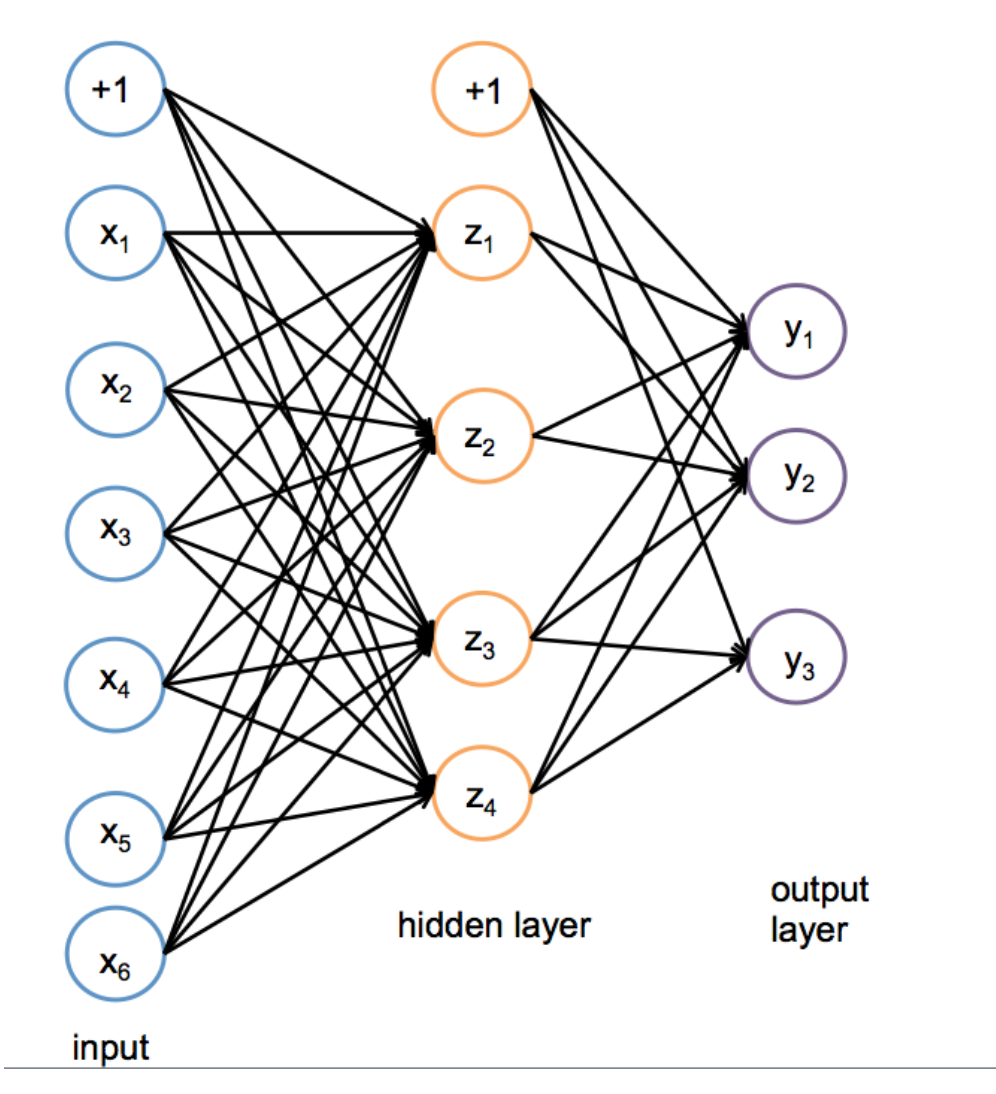
\includegraphics[width=7cm]{figure/p5.png}
    \caption{A One Hidden Layer Neural Network}
\end{figure}
\paragraph{Network Details}

Equivalently, we define each of the following. \\
The input:
$$x=[x_1,x_2,x_3,x_4,x_5,x_6]^{\top}$$

Linear combination at first (hidden) layer:
$$a_j= \alpha_{j,0} + \sum_{i=1}^6 \alpha_{j,i}*x_i,\,\, \forall j \in \{1,\ldots,4\}$$

Activation at first (hidden) layer:
$$z_j = \sigma(a_j) = \frac{1}{1+\exp(-a_j)},\,\, \forall j \in \{1,\ldots,4\}$$

Linear combination at second (output) layer:
$$b_k = \beta_{j,0} + \sum_{j=1}^4 \beta_{k,j}*z_j,\,\, \forall k \in \{1,\ldots,3\}$$

Activation at second (output) layer:
$$\hat{y}_k = \frac{\exp(b_k)}{\sum\limits_{l=1}^3 \exp(b_l)},\,\, \forall k \in \{1,\ldots,3\}$$

Note that the linear combination equations can be written equivalently as the product of the transpose of the weight matrix with the input vector. We can even fold in the bias term $\alpha_{j,0}$ by thinking of $x_0 = 1$, and fold in $\beta_{j,0}$ by thinking of $z_0 = 1$.

\paragraph{Loss}

We will use cross-entropy loss, $\ell(\hat{y},y)$. If $y$ represents our target output, which will be a one-hot vector representing the correct class, and $\hat{y}$ represents the output of the network, the loss is calculated by:
$$\ell(\hat{y},y) = - \sum_{i=1}^3 y_i \ln(\hat{y}_i)$$

\paragraph{Prediction}
When doing prediction, we will predict the $\argmax$ of the output layer. For example, if $\hat{y}_1=0.3, \hat{y}_2=0.2, \hat{y}_3=0.5$ we would predict class 3. If the true class from the training data was $2$ we would have a one-hot vector $y$ with values $y_1=0$, $y_2=1$, $y_3=0$.

(a) \defpoints{8} We initialize the weights as:
\begin{center}
$$\boldsymbol{\alpha}=
    \begin{bmatrix}
    1 & 2 & -3 & 0 & 1 & -3 \\
    3 & 1 & 2 & 1 & 0 & 2 \\
    2 & 2 & 2 & 2 & 2 & 1 \\
    1 & 0 & 2 & 1 & -2 & 2
    \end{bmatrix}$$
$$\boldsymbol{\beta}=
    \begin{bmatrix}
    1 & 2 & -2 & 1 \\
    1 & -1 & 1 & 2 \\
    3 & 1 & -1 & 1
    \end{bmatrix}
$$
\end{center}

And weights on the bias terms (${\alpha}_{j,0}$ and ${\beta}_{j,0})$ are initialized to 1.

You are given a training example $x^{(1)}=[1,1,0,0,1,1]^{\top}$ with label class 2, so $y^{(1)}=[0,1,0]^{\top}$. Using the initial weights, run the feed forward of the network over this example (without rounding during the calculation) and then answer the following questions, \textcolor{red}{round to 4 decimal places}.

(1) What is $a_1$?
\begin{tcolorbox}[fit,height=1cm, width=2cm, blank, borderline={1pt}{-2pt}]

\end{tcolorbox}

(2) What is $z_1$?
\begin{tcolorbox}[fit,height=1cm, width=2cm, blank, borderline={1pt}{-2pt}]

\end{tcolorbox}

(3) What is $a_3$?
\begin{tcolorbox}[fit,height=1cm, width=2cm, blank, borderline={1pt}{-2pt}]

\end{tcolorbox}

(4) What is $z_3$?
\begin{tcolorbox}[fit,height=1cm, width=2cm, blank, borderline={1pt}{-2pt}]

\end{tcolorbox}

(5) What is $b_2$?
\begin{tcolorbox}[fit,height=1cm, width=2cm, blank, borderline={1pt}{-2pt}]

\end{tcolorbox}

(6) What is $\hat{y}_2$?
\begin{tcolorbox}[fit,height=1cm, width=2cm, blank, borderline={1pt}{-2pt}]

\end{tcolorbox}

(7) Which class would we predict on this example?
\begin{tcolorbox}[fit,height=1cm, width=2cm, blank, borderline={1pt}{-2pt}]

\end{tcolorbox}

(8) What is the total loss on this example?
\begin{tcolorbox}[fit,height=1cm, width=2cm, blank, borderline={1pt}{-2pt}]

\end{tcolorbox}



(b) \defpoints{10} Now use the results of the previous question to run backpropagation over the network and update the weights. Use learning rate $\eta=1$.

Do your backpropagation calculations without rounding then answer the following questions, then in your responses, \textcolor{red}{round to 4 decimal places}.

(1) What is the updated value of ${\beta}_{2,1}$?
\begin{tcolorbox}[fit,height=1cm, width=2cm, blank, borderline={1pt}{-2pt}]

\end{tcolorbox}

(2) What is the updated weight of the hidden layer bias term applied to $y_1$ (i.e. ${\beta}_{1,0}$)?
\begin{tcolorbox}[fit,height=1cm, width=2cm, blank, borderline={1pt}{-2pt}]

\end{tcolorbox}

(3) What is the updated value of ${\alpha}_{3,4}$?
\begin{tcolorbox}[fit,height=1cm, width=2cm, blank, borderline={1pt}{-2pt}]

\end{tcolorbox}

(4) What is the updated weight of the input layer bias term applied to $z_2$ (i.e. ${\alpha}_{2,0}$)?
\begin{tcolorbox}[fit,height=1cm, width=2cm, blank, borderline={1pt}{-2pt}]

\end{tcolorbox}

(5) If we ran backpropagation on this example for a large number of iterations and then ran feed forward over the same example again, which class would we predict?
\begin{tcolorbox}[fit,height=1cm, width=2cm, blank, borderline={1pt}{-2pt}]

\end{tcolorbox}



(c) \defpoints{12} Let us now introduce regularization into our neural network. For this question, we will incorporate L2 regularization into our loss function $\ell(\hat{y},y)$, with the parameter $\lambda$ controlling the weight given to the regularization term. \textcolor{red}{Round your answer to 4 decimal places}

(1) Write the expression for the regularized loss function of our network after adding L2 regularization (\textbf{Hint:} Remember that bias terms should not be regularized!)
\begin{tcolorbox}[fit,height=3cm, width=10cm, blank, borderline={1pt}{-2pt}]

\end{tcolorbox}

(2) Compute the regularized loss for training example $x^{(1)}$ (assume $\lambda$ = 0.01 and use the weights before backpropagation)
\begin{tcolorbox}[fit,height=1cm, width=2cm, blank, borderline={1pt}{-2pt}]

\end{tcolorbox}

Suppose the weight initialization for $\alpha$ is changed to the following:
$$\boldsymbol{\alpha}=
\begin{bmatrix}
10 & 20 & -30 & 0 & 10 & -30 \\
30 & 10 & 20 & 10 & 0 & 20 \\
20 & 20 & 20 & 20 & 20 & 10 \\
10 & 0 & 20 & 10 & -20 & 20
\end{bmatrix}$$

$\beta$ and bias terms are not changed. \\

(3) Report the non-regularized loss for the network on training example $x^{(1)}$
\begin{tcolorbox}[fit,height=1cm, width=2cm, blank, borderline={1pt}{-2pt}]

\end{tcolorbox}

(4) Report the regularized loss for the network on training example $x^{(1)}$ ($\lambda$ = 0.01)
\begin{tcolorbox}[fit,height=1cm, width=2cm, blank, borderline={1pt}{-2pt}]

\end{tcolorbox}

(5) For a network which uses the regularized loss function, write the gradient update equation for $\alpha_{j,i}$ . You may use $\frac{\partial \ell(\hat{y},y)}{\partial \alpha_{j,i}}$ to denote the gradient update w.r.t non-regularized loss and $\eta$ to denote the learning rate.
\begin{tcolorbox}[fit,height=3cm, width=10cm, blank, borderline={1pt}{-2pt}]

\end{tcolorbox}

(6) Based on your observations from previous questions, \textbf{select all statements which are true}:
\begin{list}{}
    \item $\square$ The non-regularized loss is always higher than the regularized loss
    \item $\square$ As weights become larger, the regularized loss increases faster than non-regularized loss
    \item $\square$ On adding regularization to the loss function, gradient updates for the network become larger
    \item $\square$ When using large initial weights, weight values decrease more rapidly for a network which uses regularized loss
    \item $\square$ None of the above
\end{list}